\documentclass[a4paper,11pt]{jsarticle}
\usepackage{amsthm} %定理系を入れるのに必須
\usepackage{amsmath,amssymb} %\dfrac
\usepackage{bm} %\bm:斜体太字の文字を書けるようにする(ベクトル表記)
\usepackage{ascmac} %参考http://akita-nct.jp/yamamoto/comp/latex/make_doc/box/box.php
\usepackage{fancyhdr} %ヘッダに任意の文字列を書く
\usepackage{amsfonts} %\mathbb:白抜き文字を書けるようにする
\usepackage{enumerate}
\usepackage[english]{babel}

\usepackage[dvipdfmx]{graphicx} %図表を入れる場合
\usepackage{float} %図表の位置
\usepackage{subfigure}



\makeatletter
   \renewcommand{\theequation}{%
   \thesection.\arabic{equation}}
   \@addtoreset{equation}{section}
\makeatother

\theoremstyle{definition}
\newtheorem{theorem}{Thm.}[subsection] 
\newtheorem{definition}{Def.}[subsection]
\newtheorem{lem}{Lem.}[subsection]
\newtheorem{prf}{Prf.}[subsection]
\newtheorem{prop}{Prop.}[subsection]
\newtheorem{ex}{Ex.}[subsection]
\newtheorem{asm}{Asm.}[subsection]

%ナンバリングを外したいとき
\newtheorem*{theorem*}{Thm.} 
\newtheorem*{definition*}{Def.}



%偏微分,チルダ,分数
\newcommand{\pd}[2]{\dfrac{\partial #1}{\partial #2}}
\newcommand{\pdd}[2]{\dfrac{{\partial}^2 #1} {\partial {#2}^2} }
\newcommand{\ti}[1]{\tilde{#1}}
\newcommand{\df}[2]{\dfrac{#1}{#2}}
\newcommand{\intinf}{\int_{-\infty}^{\infty}}

\title{Advanced Derivative}
\author{Kohei Fukushima}
\date{\today}

\begin{document}
\maketitle
\pagestyle{fancy}
\lhead{Advanced Derivative}
%\rhead{\today}
\rhead{\rightmark}



% \newpage
% \thispagestyle{empty}
% \tableofcontents %目次

\section{Bond and Forward Contract}
\subsection{Interest Rates}
\begin{asm}
  We asssume that there exists a default free
  money market account
  \begin{itemize}
    \item default-free
    \item liquid (borrowing ragte = lending rate)
    \item everyone can access equally
  \end{itemize}
\end{asm}

The interest rates associating with the default free m.m.
(money market) are called risk-free rates.


\subsubsection{Types of Accrual (利息)}
Suppose one invests cash amount $A$ at $t=0$ for $T$ years. \\
$V$ : The amount of cash to be returned in $T$ years time.

\begin{enumerate}
  \item Annual compounding with interest rate $R_1$ per annum\\
  $V=A(1+R_1)^T$
  \item Semiannual compounding with interest rate $R_2$ per annum\\
  $V=A(1+\frac{R_2}{2})^{2T}$
  \item m-times compounding with interest rate $R_m$ per annum\\
  $V=A(1+\frac{R_m}{m})^{mT}$
  \quad (typiccaly we have $m=1,2,4,12,52,365$)
  \item continuous compounding with interest rate $r$ per annum\\
  $V=\lim_{m\to\infty}A(1+\frac{r}{m})^{mT}=Ae^{rT}$  
\end{enumerate}

Relation among different compounding conventions:

\underline{No-Arbitrage}
\quad $\to$ for any $m$, 
\begin{align}
  e^{rT}&=\left(1+\df{R_m}{m}\right)^{mT} \\
  \Leftrightarrow \quad r&=m \ln\left(1+\df{R_m}{m}\right),
  \quad R_m=m(e^{r/m}-1).
\end{align}

at a given time, $R_1(T)$ : $T$ dependent. 


\subsubsection{Zero Rate and Bonds}
%https://ja.sharelatex.com/learn/Theorems_and_proofs
%http://iso.2022.jp/math/abbrev/
\begin{definition}{(zero rate)}
The T-year zero-coupon interest rate is the rate of interest 
earned on an investment that starts today and lasts for T-years
without any intermidiate coupon payment.
\end{definition}

\begin{ex}
  5-year zero rate = 5 \% per annum. (continuous compounding)\\
  \$ $100$をdeposit at $t=0$ $\to$ (5 years later) 
  $100e^{0.05\times 5} \approx 128.40 $
\end{ex}

Present value (PV) \quad
$P.V.=128.40 \times e^{-0.05\times 5} = 100 $

\begin{definition}{(ZCB : zero coupon bond)}
  T-year zero coupon bond is a bond which pays an unit amount
  of cash in T-year time without any coupon payment
  (assume risk-free, liquid).
\end{definition}

If $R$ is T-year zero rate, 
current price of T-year zero coupon Bond is given by :
\begin{align}
  P(0,T)=e^{-RT}
\end{align}
($0$: current time, $T$: maturity), \quad
we call "discount factor".

\begin{ex}\label{bondprice}
  Suppose we have (at $t=0$)
  \begin{itemize}
    \item $T=0.5, \, R=5.0\%$ \, (zero coupon rate)
    \item $T=1.0, \, R=5.8\%$
    \item $T=1.5, \, R=6.4\%$
    \item $T=2.0, \, R=6.8\%$
  \end{itemize}
  fixed coupon bond
  \begin{itemize}
    \item maturity: $T=2$
    \item coupon payments: 6\% per annum semiannually.
    \item principal: \$100
  \end{itemize}
  \begin{align}
    \mbox{Bond price}&=3P(0,0.5)+3P(0,1.0)+3P(0,1.5)+103P(0,2) \notag\\
    &=3\times e^{-5\%\times 0.5}+3\times e^{-5.8\%\times 1.0}
    +3\times e^{-6,4\%\times 1.5}+103\times e^{-6.8\%\times 2.0} \notag\\
    &\approx 98.39
  \end{align}
\end{ex} 


\subsubsection{Yield (平均利率,平均利回り,平均discount rate)}
\begin{definition}{(Bond's Yield)}
  A bond's yield is the single discount rate
  that when applied to eery cash flow,
  gives the market bond price.
\end{definition}

\begin{ex}
  using Ex. \ref{bondprice}, 
  suppose $\mbox{market price} = 98.39$ \\
  Then the yield for the bond $y$ is given by solving
  \begin{align}
    &3e^{-0.5y}+3e^{-1.0y}+3e^{-1.5y}+103e^{-2.0y} = 98.39 \\
    \Rightarrow& y \simeq 6.76\% \quad \mbox{(continuous compounding)}
  \end{align}
\end{ex}

\begin{definition}{(Par Yield)}
  The par yield for a certain maturity is the coupon rate
  that makes the bond price equal to its principal.
\end{definition}

\begin{ex}
  using Ex. \ref{bondprice}, 
  par yield $C$ for 2-year coupon bond is given by:
  \begin{align}
    &\df{C}{2}e^{-0.050\cdot 0.5}+\df{C}{2}e^{-0.058\cdot 1.0}
    +\df{C}{2}e^{-0.064\cdot 1.5}
    +\left(100+\df{C}{2}\right)e^{-0.068\cdot 2.0}=100 \\
    \Rightarrow& C\simeq 6.87\%
  \end{align}
  (par yield for $T=2$, semiannual coupon payments) \par
  In general, 
  \begin{itemize}
    \item T-year bond
    \item m-time coupon payment per annum
    \item par yield $C$
  \end{itemize}
  \begin{align}
    &\sum_{n=1}^{mT}\df{C}{m}P\left(0,\df{n}{m}\right)+100P(0,T)=100 \\
    \Rightarrow& C=\df{100(1-P(0,T))}{A}, \quad
    A=\sum_{n=1}^{mT}\df{1}{m}P\left(0,\df{n}{m}\right)
  \end{align}
\end{ex}


\subsubsection{Duration}
fixed coupond bond:
\begin{itemize}
  \item $(\mbox{cash flow at } T_i) =C_i \quad (i=1, ..., n)$
  \item $C_i$: coupon (+ principal at maturity)
\end{itemize}
Suppose its yield is given by $y$ (continuous compounding).\\
Bond price: 
\begin{align}
  B=\sum_{i=1}^{n}C_i e^{-yT_i}
\end{align}
The duration of the Bond:
\begin{align}
  D:=-\df{1}{B} \df{d}{dy} B= -\left(\df{dB/dy}{B} \right) 
  =\df{1}{B}\sum_{i=1}^{n}C_i T_i e^{-yT_i}
\end{align}

\begin{ex}{zero coupon Bond}
  \begin{align}
    &(C_i=0)_{i=1,2,...,n-1}, \, C_n=1, \quad B=e^{-yT_n}\\
    \Rightarrow& D=\df{1}{B}C_n T_n e^{-yT_n}=T_n
  \end{align}
\end{ex}

(* Durationの長短により,金利に対する反応度の違いがわかる.)

Suppose the yield changes small amount $\Delta y$, 
($y\to y+\Delta y, \quad B\to B+\Delta B$) \\
\begin{align}
  \df{\Delta B}{B}=-D\Delta y + o(\Delta y)
\end{align}
(abbr.)

Suppose $D=10$ (10 year),
yield: $\Delta y=+0.1\%$ (10 basis points, b.p.):
\begin{align}
  \df{\Delta B}{B} \approx -10 \times 0.1\% =-1\%=-0.01
\end{align}


\subsubsection{Modified Duration}
yield (m-time compounding) $\hat{y}$ \\
the same bond: 
\begin{align}
  B=\sum_{i=1}^{n}C_i \left(1+\df{\hat{y}}{m}\right)^{-mT_i}  
\end{align}
modified duration:
\begin{align}
  D^{*}:&=-\df{1}{B} \df{dB}{d\hat{y}}
  =\df{1}{B}\sum_{i=1}^{n}\df{C_i T_i}{1+\hat{y}/m}
  \left(1+\df{\hat{y}}{m}\right)^{-mT_i} \notag\\
  &=\df{1}{B(1+\hat{y}/m)}\sum_{i=1}^{n}C_i T_i
  \left(1+\df{\hat{y}}{m}\right)^{-mT_i} \notag\\
  &=\df{1}{B(1+\hat{y}/m)}\sum_{i=1}^{n}C_i T_i e^{-yT_i}
  =\df{D}{1+\hat{y}/m} \quad (\mbox{no arbitrage})
\end{align}
* durationの議論はcash flowが一方向のときのみ使える.
Insuranceでは通用しないので注意.


\subsubsection{Convexity}
$y$ : yiled (continuous compounding)
\begin{align}
  C:=\df{1}{B}\df{d^2B}{dy^2}
  =\df{1}{B}\sum_{i=1}^{n}C_i T_i^2 e^{-yT_i}
\end{align}
$y\to y+\Delta y, \quad B\to B+\Delta B$:
\begin{align}
  &\Delta B=\df{dB}{dy}\Delta y
  +\df{1}{2}\df{d^2B}{dy^2}(\Delta y)^2+o(\Delta y^2) \\
  \Rightarrow&\df{\Delta B}{B}=-D\Delta y
  +\df{1}{2}C(\Delta y)^2+o(\Delta y^2) 
\end{align}

(Duration matching : abbr.)



\subsection{Forward Contract}
\subsubsection{Forward Price}

\begin{definition}{(Forward Contract)}
  A forward contract with maturity $T$ is a bilateral binding
  promise(agreement) such that at time $t=T(>0)$,
  the two parties exchange:
  \begin{itemize}
    \item the cash amount given by the time $T$ realization of
    a certain index (such as a stock price) with the fixed amount of
    cash (cash delivery)
    \item the unit amount of asset (such as a share of an equity)
    with fixed amount of cash (physical delivery=現物)
  \end{itemize}
\end{definition}

\begin{definition}{(Forward Price)}
  A forward price $F$ at the current time ($t=0$) (契約時) of
  the underlying index $X$ is the amount of cash $K$ that make
  the present value of the forward contract exchanging $X_t$
  and $K$ at $T$ zero. 
  (Forward contract has $P.V.=0$, with $K=F$.)\\
  * $F$は契約時に支払う額ではないことに注意(元手は不要) \\
  * $K$ such that P.V. of the fwd contract $=0$
\end{definition}

\begin{ex}\label{fwd1}
  Consider a forward contract on a non-dividend paying stock,
  with mat. $T$.
  
  $X_T=S_T$ (stock price at $T$),
  exchange $F \leftrightarrow S_T$ (at $T$).
  \begin{asm}
    Stock market is liquid, zero-coupon bond is liquid.
  \end{asm}
  the forward price at $t=0$ is given by:
  \begin{align}
    F=\df{S_0}{P(0,T)}=e^{rT}S_0
  \end{align}
  \begin{itemize}
    \item $r$ : zero-rate for mat $T$, continuous, compounding
    \item $P(0,T)$ : zero coupon bond price
  \end{itemize}
  
  \begin{prf}{replication strategy}
    \begin{itemize}
      \item Enter the fwd contract to get one share of stock
      ($S_T$) by paying $F$ at $T$
      ($t=0$でenterする際に元手は不要)
      \item Sell one share of stock at $t=0$ to get $S_0$
      (short position)
      \item Use $S_0$ to buy ZCB (zero coupon bond) by the amount
      $S_0/P(0,T)$
      \item Pay $F$ and receive $S_T$ at $T$ (return $S_T$ to lender)
      \item Receive $S_0/P(0,T)$ from ZCB lender
    \end{itemize}
    (cash flow illustration below) \\
    if $F\neq \df{S_0}{P(0,T)} \Rightarrow$ arbitrage
    (no risk, arbitrary positive return) \\
    No-arbitrage $\Rightarrow F=\df{S_0}{P(0,T)}=e^{rT}S_0$
    ($F$はstochasticではない)
  \end{prf}
\end{ex}

\begin{figure}[H] %HはHereを意味する
  \begin{center}
    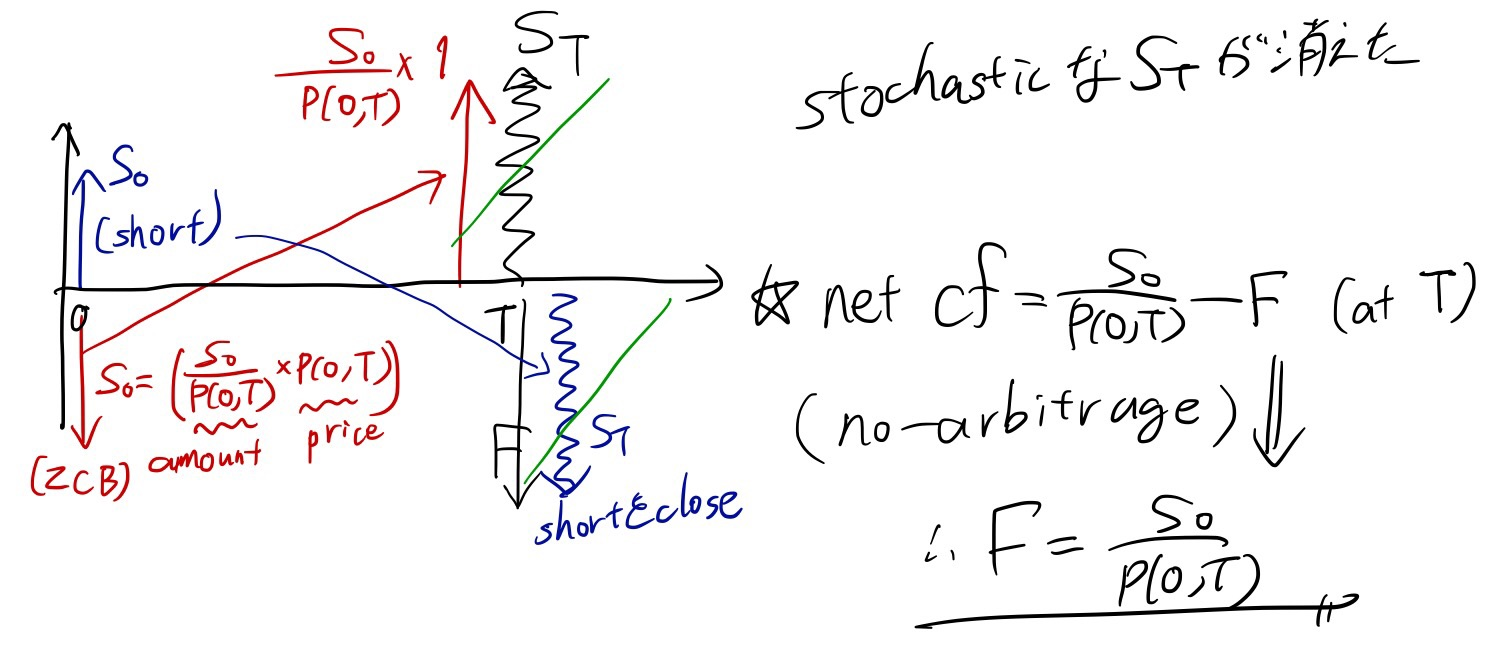
\includegraphics[width=10cm]{fig/1_2_01.JPG}
  \end{center}
\end{figure}


\begin{ex}
  Same as Ex.\ref{fwd1} but now the stock pays 
  \underline{continuous dividend}, with dividend rate $y$
  ($y\in \mathbb{R}$, constant)

  One share of the stock pays $S_t ydt$ for the interval
  $[t, t+dt]$ for any $t\geq 0$. \\
  \underline{forward price at $t=0$}
  \begin{align}
    F=\df{S_0}{P(0,T)}e^{-yT}=S_0 e^{(r-y)T}
  \end{align}
  $r$ : zero-rate for mat $T$ at $t=0$

  Suppose we heve $N_t$ shares at $t$,
  dividend paid in $[t, t+dt]: \, S_t N_t ydt$ \\
  $\Rightarrow$ reinvest $\Delta N_t = N_t ydt$

  if one reinvests the whole dividend payment, 
  \begin{align}
    \df{dN_t}{dt}=N_t y \, \Rightarrow \,
    N_t=N_0e^{yt} \quad \mbox{for all} \quad t\geq 0
  \end{align}
  Therefore, if one wants $N_T=1$, $N_0$ is to be $e^{-yT}$.

  \begin{prf}{replication strategy} \\
    ($t=0$)
    \begin{itemize}
      \item Enter the fwd contract to receive $F$ and deliver
      one share stock at $T$ (Ex.\ref{fwd1} と逆のparty)
      \item Sell $\df{S_0 e^{-yT}}{P(0,T)}$ amount of ZCB with maturity $T$
      \item Buy $e^{-yT}$ shares of stock
    \end{itemize}
    (always)
    \begin{itemize}
      \item Reinvest every div. payment to the stock
    \end{itemize}    
    ($t=T$)
    \begin{itemize}
      \item Receive $F$, deliver one share of stock
      \item Return $\df{S_0 e^{-yT}}{P(0,T)}$ to the ZCB lender
    \end{itemize}
    (cash flow illustration below)
  \end{prf}
\end{ex}

\begin{figure}[H] %HはHereを意味する
  \begin{center}
    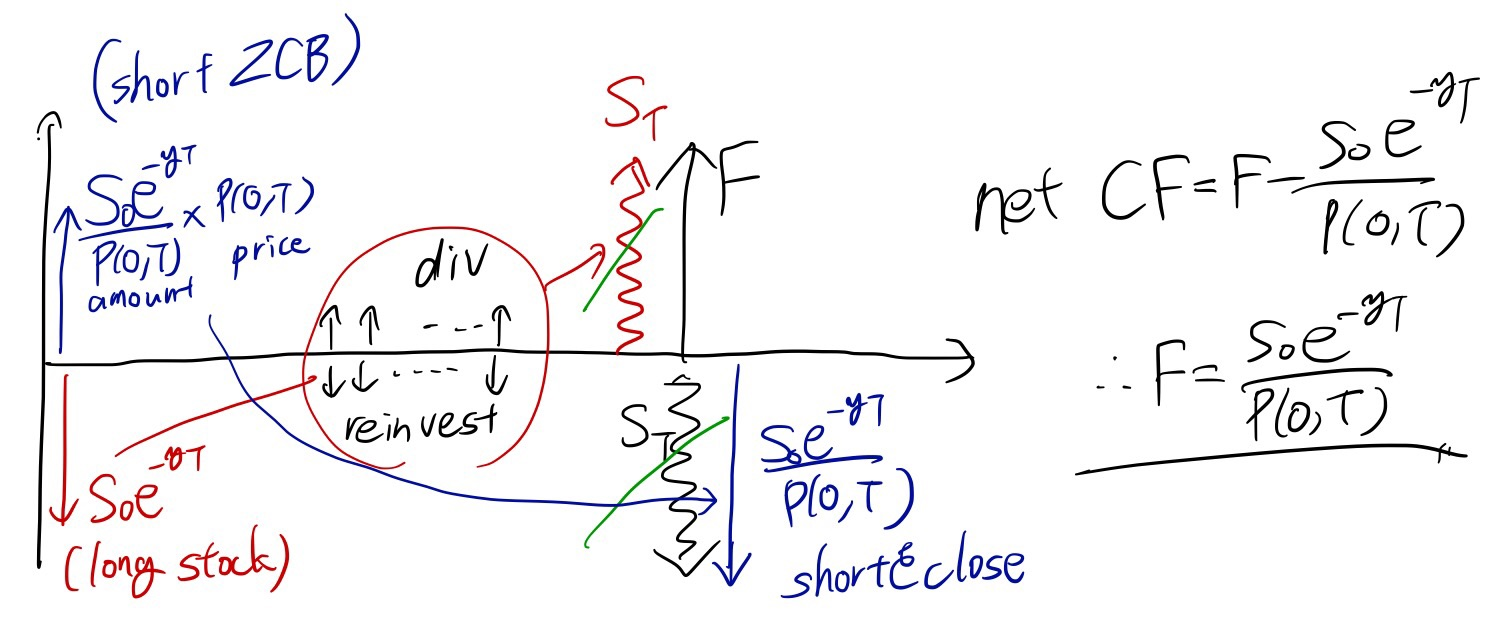
\includegraphics[width=10cm]{fig/1_2_02.JPG}
  \end{center}
\end{figure}

イメージ:
\begin{align}
  \mbox{P.V}(\mbox{receive} \, S_T \,\mbox{at} \, T)
  =F\times P(0,T)=\df{S_0}{P(0,T)}\times P(0,T)=S_0
\end{align}

randomなcash flowのP.V.を計算するときは,Forward Priceを求めて,
$P(0,T)$を乗じてやればよい(ただし市場がliquid,replicatableなときのみ)

$\Rightarrow$ 後にrisk-nuetralの下で計算すればわざわざreplicationを考える必要がなくなる


\subsubsection{Mark to Market of a Fwd Contract}
* P.V.(at $t=0$)\{fwd contract\}は0だが,時間が進むにつれて,
P.V.は変化する.

Suppose we entered the fwd contract to receive $X_T$
in exchange for a fixed amount of cash $F_0$
($F_0$ : fwd price at $t=0$). P.V.($t=0$)$=0$ \\
at time $t\in(0,T)$, suppose fwd price is given by $F_t$.
We want to know P.V.($t>0$).\\
Ans.:
\begin{align}
  \mbox{P.V.}(t)=P(t,T)(F_t-F_0)
\end{align}
\begin{prf}
  enter the new fwd contract at $t=t$
  (pays $X_T$ and receives $F_t$ at $t=T$) \\
  * $F_t$の$t$は「時刻$t$にcontractにenterした」という意味.

  (abbr.)
  \begin{align}
    \mbox{P.V.}(\mbox{at}\, t)
    \{\mbox{new + original fwd contracts}\}
    &=P(t,T)(F_t-F_0) \notag \\
    &=0+\mbox{P.V.}(\mbox{at}\, t)\{\mbox{original}\}
  \end{align}
\end{prf}

\subsubsection{Put-Call Parity}
\begin{definition}{(Call Option and Put Option)}
  A call (respectively, put) option on a certain index $X$
  with expiry $T$ and strike $K$ is the binomial?? contract
  to pay the holder of the option the cash amount equal to
  $\max(X_T-K,0)$, (resp, $\max(K-X_T,0)$)
\end{definition}

Let $C$ (resp, $P$) be the call (resp, put) option orice
(at $t=0$). We have the following put-call parity:
\begin{align}
  C-P=P(0,T)(F_X-K)
\end{align}
- $F_X$ : the fwd price of $X$ with mat. $T$
(時刻$t=X$ではなく,underlying asset $X$ をもとにした
fwd price at $t=0$)

\begin{prf}
  cash flow at $T$:
  \begin{align}
    \max(X_T,K,0)-\max(K-X_T,0)=X_T-K \\
  \end{align}
  Present value of above is given by:
  \begin{align}
    C-P=P(0,T)(F_X-K)
  \end{align}
\end{prf}

motivation:
\begin{itemize}
  \item liquidityの問題
  \item call, putの一方が求まれば,もう一方をすぐに求められる
  \item PDEの計算はputの方が簡単(because of boundary condition)
\end{itemize}



\subsection{Forward Rate Agreement and Interest Rate Swap}
*金利スワップはnot tradable

\subsubsection{Simple Rate and Day-Count Convention}
Suppose $T_i$ specifies the date $D_i=D(d_i, m_i, y_i)$
\begin{enumerate}
  \item{Actual/365}
  \begin{align}
    \delta(T_0, T_1)=\df{D_1-D_0}{365}
  \end{align}
  \item{Actual/360}
  \begin{align}
    \delta(T_0, T_1)=\df{D_1-D_0}{360}
  \end{align}
  \item{30/360}
  \begin{align}
    \delta(T_0, T_1)
    =\df{\max(30-d_0,0)+\min(d_1,30)+360(y_1-y_0)
    +30(m_1-m_0-1)}{360}
  \end{align}
  \item{actual/actual} considering leap year? 365 or 366
\end{enumerate}

\begin{definition}{(Simple Rate)}
  A (risk-free) simple rate (not compound) $L(T_{i-1},T_i)$
  with day-count $\delta(T_{i-1},T_i)$ is the interest rate with
  accrual convention defined in such a way that, when one invest
  $N$ amount of cash at $T_{i-1}$, then he receives
  $N(1+\delta_i L(T_{i-1},T_i))$ at time $T_i$.
  $L(T_{i-1},T_i)$ is the zero coupon rate at $T_{i-1}$
  for $[T_{i-1},T_i]$ with corresponding day-count convention.
\end{definition}
*accrual: ??

\subsubsection{Forward Rate Agreement (FRA)}
\begin{definition}{(Forward Rate Agreement)}
  A FRA is a binding(義務の) contract with the two parties
  (lender and borrower) agreeing to let a certain fixed rate $K$
  act on a prefixed notional(想定元本)
  amount $N$, over a future period
  $[T_M, T_N]$.
\end{definition}
*notional: 想定される?

\begin{definition}{(Forward Rate)}
  A forward rate $F$ for the period $[T_M,T_N]$ with day-count
  $\delta=\delta(T_M,T_N)$ is the fixed rate $K$ with the some
  day-count convention that makes the present value of the FRA zero.
\end{definition}

off course,
\begin{align}
  F=L(T_M, T_N) \quad (\mbox{at} \, T_M)
\end{align}
*$L$ : simple rate

\begin{lem}
  Let $\delta=\delta (T_M,T_N)$. Then the forward rate $F$
  at $t=0$ fot the period $[T_M,T_N]$ is given by
  \begin{align}
    F=\df{1}{\delta}\left(\df{P(0,T_M)}{P(0,T_N)}-1\right)
  \end{align}
  (*asm: liquid, no-arbitrage)

  \begin{prf}{replication strategy}
    \begin{itemize}
      \item Enter the FRA of rate $F$ to borrow
      unit amount of cash for $[T_M,T_N]$
      \item Sell one ZCB with mat. $T_N$ (short)
      \item Buy ZCB with mat. $T_N$ with principal amount
      $\df{P(0,T_M)}{P(0,T_N)}$
      \item At $T_M$, borrow unit amount of cash through FRA
      and use it to return ZCB
      \item At $T_N$, receive the principal $\df{P(0,T_M)}{P(0,T_N)}$,
      and pays $(1+\delta F)$
    \end{itemize}
    
    Net cash flow at $T_N$:
    $\left(\df{P(0,T_M)}{P(0,T_N)}\right)-(1+\delta F)$ \\
    If we require no-arbitrage, 
    \begin{align}
      \left(\df{P(0,T_M)}{P(0,T_N)}\right)-(1+\delta F)=0
      \quad \Rightarrow \quad
      F=\df{1}{\delta}\left(\df{P(0,T_M)}{P(0,T_N)}-1\right)
    \end{align}
  \end{prf}
\end{lem}

\begin{figure}[H] %HはHereを意味する
  \begin{center}
    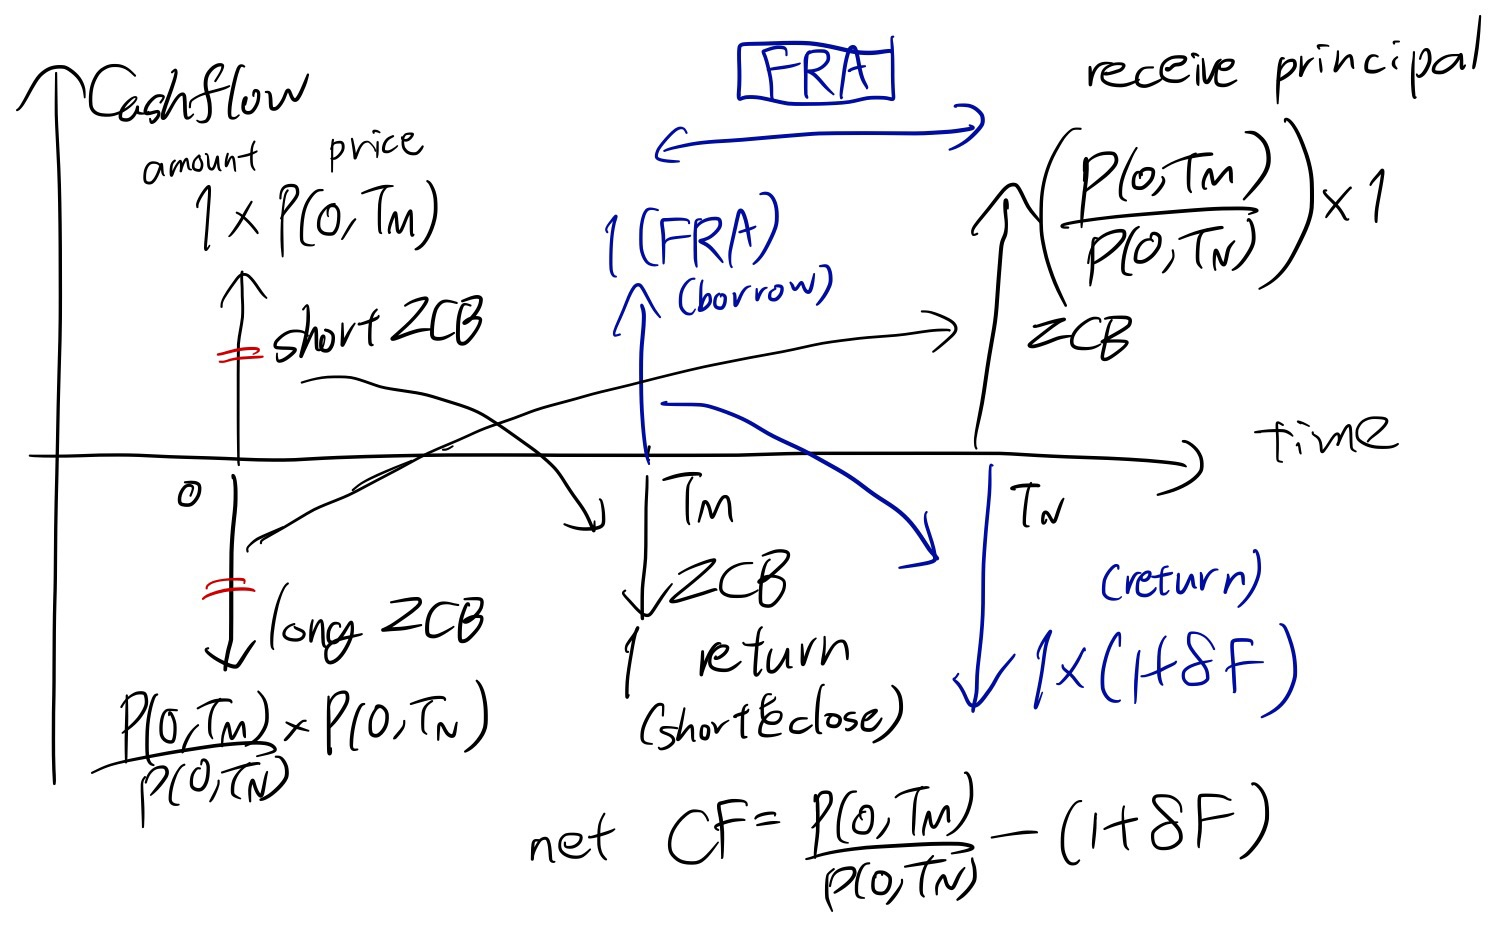
\includegraphics[width=10cm]{fig/1_3_01.JPG}
  \end{center}
\end{figure}


We write the above $F$ as
\begin{align}
  F(0,T_M,T_N)=\df{1}{\delta}\left(\df{P(0,T_M)}{P(0,T_N)}-1\right)
\end{align}
In general. at $t<T_M$,
\begin{align}
  F(t,T_M,T_N)=\df{1}{\delta}\left(\df{P(t,T_M)}{P(t,T_N)}-1\right)
\end{align}
$t\uparrow T_M$:
\begin{align}
  F(T_M,T_M,T_N)=\df{1}{\delta}\left(\df{1}{P(T_M,T_N)}-1\right)
  =L(T_M,T_N)
\end{align}

($\because$)
\begin{align}
  1=P(T_M,T_N)\{1+\delta L(T_M,T_N)\}
\end{align}
at $T_M$ invest 1, at $T_N$ return $1+\delta L(T_M,T_N)$ \\
(otherwise there exist arbitrage opportunities.) \\
(abbr.)

\begin{ex}
  Q) P.V.(at $0$) \{receive $1+\delta L(T_M,T_N)$\} ?
  $\rightarrow$ A) P.V.=0 \\
  ($\because$)
  Suppose that we are at $t=T_M$, $L(T_M,T_N)$ ... known 
  \begin{align}
    \mbox{P.V.}(\mbox{at} \, T_M)=-1+P(T_M,T_N)(1+\delta L(T_M,T_N))=0
  \end{align}
  将来のある時点($t=T_M$)でP.V.$=0$なら,さかのぼった
  $t=0$でも当然P.V.$=0$
  \begin{align}
    P.V.(\mbox{at} \, 0)\{\mbox{receive}\,
    1+\delta F(0,T_M,T_N) \, \mbox{at} \, T_N\}
    &= P.V.(\mbox{at} \, 0) \{\mbox{receive} \,
    1+\delta L(T_M,T_N)\} \\
    ( \therefore ) \quad
    P(0,T_N)F(0,T_M,T_N)&=P.V.(\mbox{at} \, 0)
    \{ \mbox{receive} \, L(T_M,T_N)  \}
  \end{align}
\end{ex}


\subsubsection{Fixed vs Floating Interest Swap}
Fix a time partition $0=T_0<T_1<...<T_M$

\begin{definition}{(Spot-start Swap)}
  A spot-start swap with maturity $T_M$ and notional amount
  $N$ is the contract in which one party (receiver)
  receives cash amount $NK\Delta_i$ ($K$ fixed)
  and pays the stochastic amount
  $NL(T_{i-1},T_i)\delta_i$ at every $T_i, \, i=\{1,2,...,M\}$.
  The other party (payer) has the opposit cash flow. Here,
  \begin{align}
    \begin{cases}
      \Delta_i &= \Delta(T_{i-1},T_i) \quad \mbox{(fixed)}\\
      \delta_i &= \delta(T_{i-1},T_i) \quad \mbox{(floating)}
    \end{cases}
  \end{align}
  are the day counts fot a fixed and floating payments, respectively.
\end{definition}

\begin{figure}[H] %HはHereを意味する
  \begin{center}
    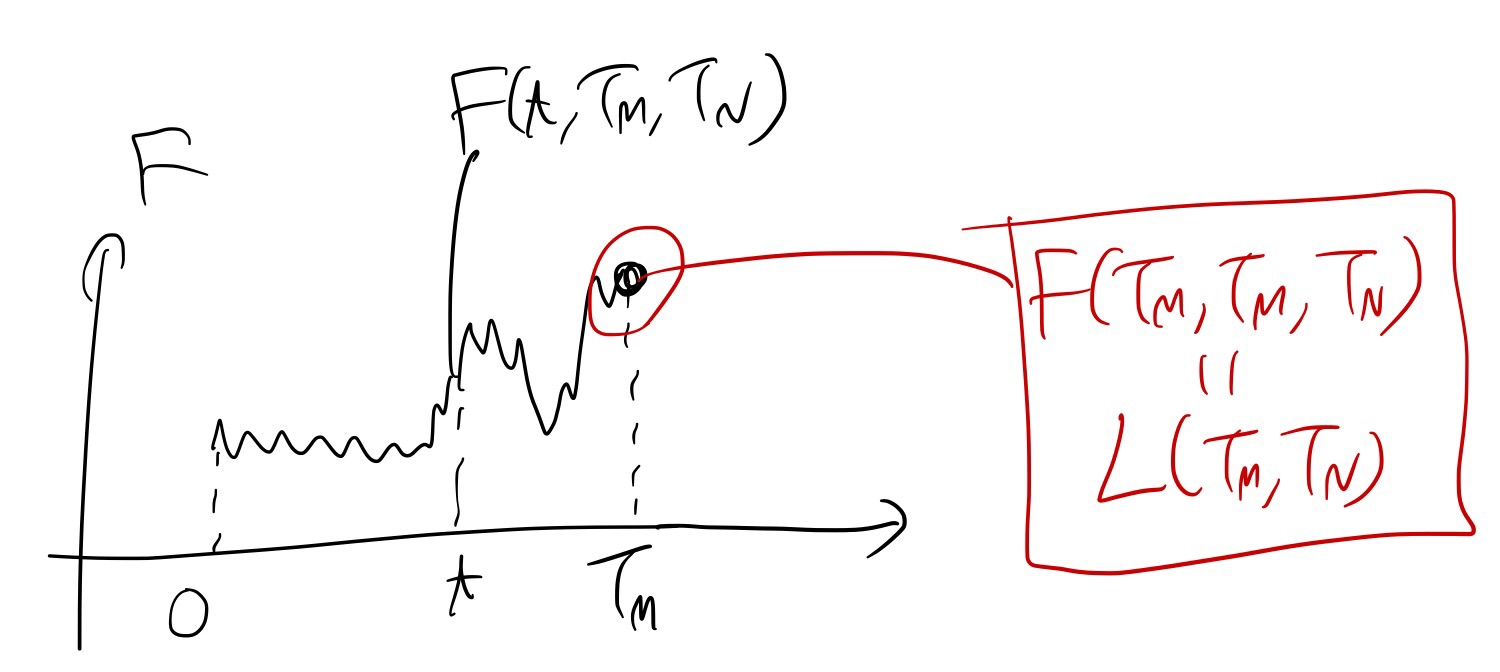
\includegraphics[width=10cm]{fig/1_3_02.JPG}
  \end{center}
\end{figure}


\begin{definition}{(Swap Rate)}
  The (spot) swap rate for the maturity $T_M$ is the fixed rate $K$
  that makes the present value of the swap zero.
\end{definition}

P.V. of the swap rate:
\begin{align}
  PV_{fix}&=NK\sum_{i=1}^M P(0,T_i)\Delta_i \\
  PV_{float}&=N\sum_{i=1}^M P(0,T_i)F(0,T_{i-1},T_i)\delta_i
  =N\sum_{i=1}^M P(0,T_i)
  \left(\df{P(0,T_{i-1})}{P(0,T_i)}-1\right) \notag \\
  &=N\sum_{i=1}^M (P(0,T_i)-P(0,T_i))
  =N(1-P(0,T_M))
\end{align}

Swap rate $K$:
\begin{align}
  K=\df{1-P(0,T_M)}{\sum_{i=1}^M P(0,T_i)\Delta_i}
  :=S(0;T_0,T_M)
\end{align}

* Economic meaning of swap rate:
\begin{align}
  S(0;T_0,T_M)
  =\df{\sum_{i=1}^M P(0,T_i)F(0,T_{i-1},T_i)\delta_i}
  {\sum_{i=1}^M \Delta_i P(0,T_i)}
\end{align}
Let us approximate as
\begin{align}\label{swap_fwd}
  P(0,T_i)\approx 1, \, \delta_i\approx\Delta_i
  \quad \mbox{for all} \, i \\
  \Rightarrow
  S(0;T_0,T_M)\approx\df{\sum_{i=1}^M F(0,T_{i-1},T_i)}{M} 
\end{align}
...average of fwd rates!

\begin{definition}{(Forward Swap)}
  A forward swap is the swap which starts at some future time.
  Fixed rate (fixed at $t=0$) which make the P.V. of the swap
  is called the forward swap rate.
\end{definition}

\begin{ex}
  A forward swap for the period $[T_M,T_N]$ \\
  $\Rightarrow$ cash flow exchanges
  at $T_i, \, i=\{M+1, ..., N\} $ \\
  $NK\Delta_i \, \leftrightarrow \, NL(T_{i-1},T_i)\delta_i$

  Let fixed rate be $K$, notional $=1$
  \begin{align}
    PV_{fix}&=NK\sum_{i=M+1}^N P(0,T_i)\Delta_i \\
    PV_{float}&=N\sum_{i=M+1}^N P(0,T_i)F(0,T_{i-1},T_i)
    \delta_i = P(0,T_M)-P(0,T_N)
  \end{align}
  Fwd Swap Rate:
  \begin{align}
    S(0;T_M,T_N)
    =\df{P(0,T_M)-P(0,T_N)}{\sum_{i=M+1}^N P(0,T_i)\Delta_i}
  \end{align}
\end{ex}


\subsubsection{Relation to the Fixed Coupon Bond}
Consider the spot-start swap for $[T_0=0, T_N]$ (notional$=0$)
\begin{align}
  PV_{float}=\sum_{i=1}^N \delta_i P(0,T_i)F(0,T_{i-1},T_i)
  =1-P(0,T_N)
\end{align}
(abbr.)


Bond-Swap, Fixed vs Floating swap, 
???

defined $i(t)$ : index, $i\in\{0,...,N\} $
s.t. $t\in[T_i,T_{i+1}) \quad T_{i(t)}\leq t < T_{i(t)+1}$

\underline{current time $t$}
\begin{align}
  &\mbox{P.V.(floating leg?+ final principal)} \notag \\
  =&P(t,T_{i(t)+1})\delta_{i(t)+1}L(T_{i(t)},T_{i(t)+1})
  +\sum_{j=i(t)+2}^N P(t,T_j)\delta_j F(t,T_{j-1},T_j)
  +P(t,T_N) \notag \\
  =&P(t,T_{i(t)+1})\delta_{i(t)+1}L(T_{i(t)},T_{i(t)+1})
  +\sum_{j=i(t)+2}^N P(t,T_j)(1+\delta_{i(t)+1}L(T_i,T_{i+1}))
  +P(t,T_N) \notag \\
  =&P(t,T_{i(t)+1})(1+\delta_{i(t)+1}L(T_i,T_{i+1}))
  \approx 1
\end{align}

Thus, floating leg + final principal $\approx$ IR-RISK $0$

IR-Swap Risk $\approx$ fixed leg + final principal payment \\
$\Leftrightarrow$ fixed coupon Bond


\subsubsection{Yield Curve Construction (Simplified...)}
\begin{asm}
  There are market quotes of spot-starting swaps with swap rate
  $\{S_n\}_{n=1}^N$ with corresponding maturities $\{T_n\}_{n=1}^N$
  \begin{align}
    S_n:S(0;T_0,T_n), \quad T_0=0
  \end{align}
\end{asm}


\begin{ex}
  3 month. $0=T_0<T_1<...<T_N$
\end{ex}
We want to get $\{P(0,T_n)\}_{n=1}^N$ which are consistent with
the swap quotes.

1) Determin $P(0,T_1)$
\begin{align}
  S_1 \Delta_1 P(0,T_1)=P(0,T_0)-P(0,T_1) \\
  S_1 = \df{1-P(0,T_1)}{\Delta_1 P(0,T_1)} \\
  P(0,T_1)=\df{P(0,T_0)}{1+\Delta_1 S_1}=\df{1}{1+\Delta_1 S_1}
\end{align}

2) Suppose we have obtained $\{P(0,T_n)\}_{n=1}^{m-1}$.
Consider $T_m$-maurity swap:
\begin{align}
  S_m \Delta_m P(0,T_m)+S_m \sum_{n=1}^{m-1} \Delta_n P(0,T_n)
  =1-P(0,T_m) \\
  \Rightarrow \, (*) \quad
  P(0,T_m)=\df{1-S_m\{\sum_{n=1}^{m-1}\Delta_n P(0,T_n)\}}
  {1+\Delta_m S_m}
\end{align}
using
\begin{align}
  (*) \quad S_m=S(0;T_0,T_m)
  =\df{\sum_{n=1}^{m}\Delta_n P(0,T_n)}{1-P(0,T_m)}
\end{align}

yield curve ... to be interpolated


\subsubsection{Mark-to-Market of a Forward Swap}
Suppose has swap starting $T_M$ with maturity $T_N$
as a receiver (long bond party) with the fixed rate $X$,
notional $L$.
Suppose the current $(t=0)$ market quotes is given by
$S(0,T_M,T_N)$.

*notional $L$はsimple rateの$L(T_{i-1},T_i)$とは別物.

\begin{align}
  PV(t=0) &= LX\sum_{n=M+1}^N \Delta_n P(0,T_n)
  -L\sum_{n=M+1}^{N}P(0,T_n)\delta_n F(0,T_{n-1},T_n)
  \notag\\
  &=L\left(\sum_{n=M+1}^{N}\Delta_n \right)
  P(0,T_n)(X-S(0,T_M,T_N))
\end{align}
bondのreceiverは金利が下がったら嬉しい

\subsubsection{Approximation of a Fwd Swap Rate}
\begin{align}
  S(0,T_M,T_N)&=\df{P(0,T_M)-P(0,T_N)}
  {\sum_{i=M+1}^N \Delta_i P(0,T_i)}
  =\df{\sum_{i=M+1}^N \delta_i F(0,T_{i-1},T_i)P(0,T_i)}
  {\sum_{i=M+1}^N \Delta_i P(0,T_i)} \notag \\
  &\approx \df{1}{N-M} \sum_{i=M+1}^N F(0,T_{i-1},T_i)
  \quad (\mbox{as } \delta_i\approx\Delta_i, \, P(0,T_i)=1)
\end{align}
... Swap rate is the average of fwd rates.

\begin{align}
  \sum_{i=M+1}^N F(0,T_{i-1},T_i)
  &=\sum_{i=1}^N F(0,T_{i-1},T_i)-\sum_{i=1}^M F(0,T_{i-1},T_i) \notag\\
  &\approx NS(0;T_0,T_N) - MS(0;T_0,T_M) \quad
  (\because \ref{swap_fwd})
\end{align}

$0<T_M<T_N$:
\begin{align}
  NS(0;T_0,T_N)\approx MS(0;T_0,T_M)+(N-M)S(0;T_M,T_N)
\end{align}
$NS(0;T_0,T_N)\approx$ \{$[T_0,T_N]$のfwd rateのsum\}

\begin{align}
  \therefore \, S(0;T_M,T_N) &\approx
  \df{NS(0;T_0,T_N)-MS(0;T_0,T_M)}{N-M} \notag \\
  &\approx \df{T_N}{T_N-T_M}S(0;T_0,T_N)
  -\df{T_M}{T_N-T_M}S(0;T_0,T_M)
\end{align}


\subsubsection{Delas (PV01s)}
* market quotes (input) spot-swap rates $(S_n)_{n=1}^N$
$\Rightarrow$ $P(0,T)$ $\Rightarrow$ pricing...

\begin{definition}{(Deltas (PV01s))}
  Deltas are the price sensitivities of a trade (or portfolio)
  against the change of each swap rate $S_n\, n=1,...,N$
\end{definition}

P.V. of portfolio\{$S_n+1b.p.,\, (S_m)_{m\neq n}^N$:unchanged\}
$-$ P.V. of portfolio\{$S_n, \, (S_n)_{n=1}^N$\}

ex. Deltas for a swap \\
Consider a fwd swap for $[T_M,T_N]$. 
Notional: $L$, fixed rate: $X$

P.V. of receiver swap $[T_M, T_N]$ :
\begin{align}
  P.V.(t=0)=L\sum_{i=M+1}^N\Delta_i P(0,T_i)(X-S(0;T_M,T_N))
\end{align}
Suppose the market change induces
\begin{align}
  S(0;T_M,T_N) \, \rightarrow \, S(0;T_M,T_N) + \delta S
\end{align}
then, change of the P.V. :
\begin{align}
  \delta P.V.=&L\sum_{i=M+1}^N\Delta_i(\delta P(0,T_i))
  (X-S(0;T_M,T_N)) \notag \\
  &+L\sum_{i=M+1}^N\Delta_i P(0,T_i)
  (-\delta S_{M,N}) + \mbox{higher order}
\end{align}

1st term order $\sim$ $IR^2$ (*IR:interest rate)\par
2nd term order $\sim$ $IR^1$ \\
$||\mbox{1st term}|| << ||\mbox{2nd term}||$

\begin{align}
  \delta P.V. \approx L\sum_{i=M+1}^N\Delta_i P(0,T_i)
  (-\delta S_{M,N})
\end{align}
* $(-\delta S_{M,N})$ : fwd swap rateの変化


\begin{align}
  S(0;T_M,T_N)&\approx\df{T_N}{T_N-T_M}S(0;T_0,T_N)
  -\df{T_M}{T_N-T_M}S(0;T_0,T_M) \\
  \delta S_{M,N}&\approx\df{T_N}{T_N-T_M}\delta S_N
  -\df{T_M}{T_N-T_M}\delta S_M
\end{align}

\begin{itemize}
  \item $\delta S_N$ : change of $S(0,T_0,T_N)$
  \item $\delta S_M$ : change of $S(0,T_0,T_M)$ 
\end{itemize}

\begin{align}
  &\delta P.V. (\mbox{fwd swap} \, (T_M,T_N)) \notag\\
  \approx& -L\sum_{i=M+1}^N\Delta_i P(0,T_i)
  \left\{\df{T_N}{T_N-T_M}\delta S_N
  -\df{T_M}{T_N-T_M}\delta S_M \right\} \notag \\
  \approx&-L(T_N-T_M)\times \df{1}{T_N-T_M}
  (T_N\delta S_N-T_M\delta S_M) \quad
  (\mbox{approx.}\, P(0,T_i)\approx 1 ) \notag \\
  \approx&-L(T_N\delta S_N-T_M \delta S_M)
\end{align}
* spot-start swap with mat. $T_N$, $T_M$のみで表せる.\\
* day-count conventionのズレは無視.

if $T_M=T_0$, replace $\delta S_M=0$

spot-start swap, maturity $T_N$, Notional $L$, receiver:
\begin{align}
  \delta P.V.=&-L\times T_N\times\delta S_N \\
  &-(\mbox{元本})\times(\mbox{duration})
  \times(\mbox{yieldの変化}) \notag
\end{align}
spot-startなら,自分がenterした年限のswap rateの変化しか関係ない.
10年swap に入る限り,5年swapや20年swapの変化は関係ない.\\
$\rightarrow$ ヘッジ戦略に使える.


\newpage
\section{Binomial Model}
多期間モデルは連続モデルへの直観を与える.
PDEの数値計算との関連もあり.

\subsection{One-Period Binomial Model}
\subsubsection{Model Description}

There are two points in time $t=0,T$.
Two tradable assets:
\begin{itemize}
  \item Bond (risk-free asset)
  \begin{align}
    B_0&=1 \\
    B_T&=e^{rT}
  \end{align}
  (deterministic) \\
  $r$: zero rate for $[0,T]$ at $T=0$
  \item Stock (risky asset)
  \begin{align}
    S_0&=s \, (>0) \\ 
    S_T&=
    \begin{cases}
      su \quad \mbox{with prob.} \, P_u \\
      sd \quad \mbox{with prob.} \, P_d
    \end{cases} \\
    &P_u>0, \, P_d>0, \, P_u+P_d=1, \, 0<d<u
  \end{align}
  We write for simplicity:
  \begin{align}
    S_T&=sZ \\
    Z&=
    \begin{cases}
      u \quad \mbox{with prob.} \, P_u \\
      d \quad \mbox{with prob.} \, P_d
    \end{cases}
  \end{align}
  under emprical measure $\mathbb{P}$, 
  $\mathbb{P}(\{up\})=P_u, \,
  \mathbb{P}(\{down\})=P_d$
\end{itemize}

Portfolio : $h(x,y) \quad x,y\in\mathbb{R}$
\begin{itemize}
  \item $x$: number of position for the bond
  \item $y$: number of position for the stock
\end{itemize}

the value process of the portfolio $h$:
\begin{align}
  V_t^h&=xB_t+yS_t \quad \mbox{in general} \\
  V_0^h&=x+ys \\
  V_T^h&=xe^{rT}+ysZ
\end{align}

\begin{definition}
  An arbitrage portfolio us a portfolio with the properties:
  \begin{align}
    V_0^h=0, \, P(V_T^h\geq 0)=1, \, P(V_T^h>0)>0
  \end{align}
  * no-arbitrage $\Leftrightarrow$ existence of risk neutral measure
  (we'll see later)
\end{definition}

\begin{prop}\label{prop_af}
  The one-period binomial model is arbitrage free
  iff (=if and only if) the following condition holds:
  \begin{align}\label{cond_af}
    0 < d < e^{rT} <u
  \end{align}

  \begin{prf}{(proof of above prop.)} 
    
    \begin{itemize}
      \item (necessarity = only if):
      Suppose \ref{cond_af} does not hold.
      \begin{enumerate}
        \item $e^{rT}\leq d < u$
        \begin{enumerate}
          \item Sell the bond $s$ units
          \item Buy one unit of the stock
        \end{enumerate}
        $h(x,y)=(-s,1)$, net cash flow $=0$ at $t=0$.
        Then,
        \begin{align}
          V_T^h=-se^{rT}+sZ=s(-e^{rT}+Z)
        \end{align}
        It's clear that $V_T^h \geq 0$, $P(V_T^h\geq 0)=1$.
        \begin{align}
          P(V_T^h>0)=P(Z=u)=P_u>0
        \end{align}
        $\rightarrow$ arbitrage.

        \item $d < u \leq e^{rT}$ \\
        \begin{enumerate}
          \item Sell one unit of the $s$ stock
          \item Buy the bond s units
        \end{enumerate}
        $h(x,y)=(s,-1)$, net cash flow $=0$ at $t=0$.
        Then,
        \begin{align}
          V_T^h=se^{rT}-sZ=s(e^{rT}-Z)
        \end{align}
        It's clear that $V_T^h \geq 0$, $P(V_T\geq 0)=1$.
        \begin{align}
          P(V_T^h>0)=P(Z=d)=P_d>0
        \end{align}
        $\rightarrow$ arbitrage.
      \end{enumerate}

      \item (sufficiency = if):
      Suppose \ref{cond_af} holds. \\
      Assume $V_0^h=0$ then $x+ys=0 \, \Leftrightarrow \, ys=-x$.
      \begin{align}
        &V_T^h =xe^{rT}+ysZ=x(e^{rT}-Z) \\
        &P(V_T^h\geq 0) < 1
      \end{align}
      $\rightarrow$  no-arbitrage.

    \end{itemize}
  \end{prf}

\end{prop}

\subsubsection{Risk-neutral Probability Measure}
Suppose $d<e^{rT}<u$ holds, \\
$\Rightarrow$ one can find $q_u, \, q_d \, >0$ s.t.

\begin{align}
  \begin{cases}
    q_u+q_d=1 \\
    q_d u+q_d d=e^{rT}
  \end{cases} \\
  \Rightarrow
  \begin{cases}
    q_u=\df{e^{rT}-d}{u-d} \quad (>0) \\
    q_d=\df{u-e^{rT}}{u-d} \quad (>0)
  \end{cases}
\end{align}
We define a new (and not emprical) probability measure
$\mathbb{Q}$ such that
\begin{align}
  \mathbb{Q}(Z=u)&=q_u \\
  \mathbb{Q}(Z=d)&=q_d
\end{align}
It's interesting to observe that
\begin{align}
  e^{-rT}\mathrm{E}^{\mathbb{Q}}[S_T]
  &=e^{-rT}(q_u\times su+q_d\times sd) \notag \\
  &=se^{-rT}(q_u u+q_d d)=s\,(=S_0)
\end{align}

In general,
\begin{align}
  \{\ e^{-rT}S_t \}_{t=0,T} \quad ... \, \mathbb{Q}
  \mbox{-martingale}
\end{align}

\begin{definition}{(Risk-neutral Measure)}
  The probability measure $\mathbb{Q}$ with associated
  probability $(q_u, q_d)$ satisfying the condition
  eq\eqref{cond_af} is called the risk-neutral measure.
\end{definition}

\begin{prop}
  The one-period binomial model just explained is arbitrage
  free iff there exists a risk-neutral measure
  $\mathbb{Q}$ ($q_u>0,\, q_d>0)$
\end{prop}

\begin{prf}
  arbitrage free $\Leftrightarrow$ $d<e^{rT}<u$
  ($\because$ Prop. \ref{prop_af}) \\
  \begin{align}
    &\mathbb{Q}=(q_u,q_d) \\
    &q_u=\df{e^{rT}-d}{u-d} , \quad
    q_d=\df{u-e^{rT}}{u-d} \\
    &q_u+q_d=1
  \end{align}

  If such $\mathbb{Q}$ exists, then
  \begin{align}
    & \exists q_u,q_d \, >0 \quad \mbox{s.t.}
    \begin{cases}
      q_u+q_d=1 \\
      q_u u + q_d d =e^{rT}
    \end{cases} \\
    \Rightarrow & \, d<e^{rT}<u
  \end{align}
\end{prf}

\subsubsection{Risk-neutral Pricing}
\begin{definition}{(Contingent Claim)}
  A contingent claim is any random cash flow $X_T$ at $T$
  of the form $X_T=\Phi(S_T)$ with some function $\Phi$.

  \begin{ex}{(call option with strike $K$)}
    \begin{align}
      \Phi(S_T)=\max(S_T-K,0)=(S_T-K)^{+}
    \end{align}
  \end{ex}
\end{definition}

\begin{definition}{(Replicable / Complete)}
  A given contingent claim $X$ is said to be replicatable
  (or perfectly hedgeable) if there exists a portfolio $h$
  such that $V_T^h=X_T$ with probability $1$ (under $\mathbb{P}$).
  In this case, we call $h$ a replicating portfolio of $X$.
  If all contingent claim are replicable, we say
  the market is complete. Otherwise the market is incomplete.
\end{definition}

\begin{prop}\label{prop_unique}
  Suppose that a contingent claim $X$ is replicable by
  portfolio $h$. Then, any price at $t=0$ of the claim $X$
  other than $V_0^h$ will lead to an arbitrage opportunity.
\end{prop}

\begin{prf}
  Suppose $h$ is given by $h=(x,y)$. Suppose $V_0^h\neq X_0$.
  \begin{enumerate}
    \item $V_0^h<X_0$
    \begin{itemize}
      \item Short the contingent claim $X$ (one gets $X_0$)
      \item Construct a portfolio $h(x,y)$ : $V_0^h=x+sy$
      \item Buy $(X_0-V_0^h)$ units of bond 
    \end{itemize}
    portfolio $h'=(x+X_0-V_0^h, y)$ + short position of $X$ \\
    net cash flow at $T$:
    \begin{align}
      V_T^{h'}-X_T=(X_0-V_0^h)e^{rT}+V_T^h -X_T
      =(X_0-V_0^h)e^{rT} > 0
    \end{align}  
    $\rightarrow$ arbitrage.
    \item $V_0^h>X_0$
    \begin{itemize}
      \item Buy the contingent claim $X$
      \item Short the replicating portfolio $h(x,y)$
      : $V_0^h=x+sy$
      \item Buy $(V_0^h-X_0)$ units of bond 
    \end{itemize}
    portfolio $h''=(V_0^h-X_0-x, -y)$ + long position of $X$ \\
    net cash flow at $T$:
    \begin{align}
      V_T^{h''}+X_T=(V_0^h-X_0)e^{rT}-V_T^h +X_T
      =(V_0^h-X_0)e^{rT} > 0
    \end{align}  
    $\rightarrow$ arbitrage.
  \end{enumerate}
\end{prf}


\begin{prop}
  The binomial model is complete.
\end{prop}

\begin{prf}
  Consider a general contingent claim $X$
  whose payoff at $T$ is $\Phi(S_T)$.
  $\Phi : \mathbb{R} \to \mathbb{R}$ function.
  \begin{ex}
    Call option $\Phi(S_T)=\max(S_T-K,0), \quad K\in\mathbb{R}$\\
    It suffices to construct a strategy $h=(x,y)$ s.t.
    \begin{align}
      V_T^h=
      \begin{cases}
        \Phi(su) \quad \mbox{if} \, Z=u \\
        \Phi(sd) \quad \mbox{if} \, Z=d
      \end{cases}
    \end{align}
    * terminal valueが複製元デリバティブと同じになるような
    portfolio $h$を探す.
    \begin{align}
      \begin{cases}
        e^{rT}x+suy=\Phi(su) \\
        e^{rT}x+sdy=\Phi(sd) 
      \end{cases} \\
      \Leftrightarrow
      \begin{cases}
        x=e^{-rT} \df{u\Phi(sd)-d\Phi(su)}{u-d} \\
        y=\df{1}{s} \df{\Phi(su)-\Phi(sd)}{u-d}
      \end{cases}
    \end{align}
  \end{ex}
\end{prf}


Option Pricing (Assume there is no-arbitrage opportunity)

Consider the same contingent claim $X$
with payoff $\Phi(S_T)$

The price $X_0$ at $t=0$ of the claim is given by
$X_0=V_0^h$ ($\because$ Prop.\ref{prop_unique}).
\begin{align}
  X_0&=x+sy
  =e^{-rT} \left\{\df{u\Phi(sd)-d\Phi(su)}{u-d}
  +e^{rT} \df{\Phi(su)-\Phi(sd)}{u-d} \right\} \notag \\
  &=e^{-rT} \left\{ \df{e^{rT}-d}{u-d} \Phi(su)
  + \df{u-e^{rT}}{u-d} \Phi(sd) \right\}  \\
  X_0 &=e^{-rT}\{ q_u\Phi(su)+q_d\Phi(sd) \}
  =e^{-rT}\mathrm{E}^{\mathbb{Q}}[\Phi(S_T)]
\end{align}

$(P_u,P_d)\leftrightarrow (q_u,q_d)$


\subsection{The Multi-Period Binomial Model}
\subsubsection{Model Description}
$0=t_0<t_1<...<t_N=T$

time partition:
\begin{align}
  t_i-t_{i-1}=\Delta t=\df{T}{N} \quad \mbox{for} \,
  \forall i
\end{align}
each $t_i \, i=\{0,...,N\}$, one can trade securities.

Securities:
\begin{itemize}
  \item Bond (risk-free, non-random) \\
  Bond price process:
  \begin{align}
    B_0=1, \, B_n=e^{r\Delta t} B_{n-1}=e^{rn\Delta t}
  \end{align}
  Risk-free rate $r \, (\geq 0)$ : constant

  \item Stock \\
  Stock price process:
  \begin{align}
    &S_0=s, \, S_n=S_{n-1}Z_n \\
    &\begin{cases}
      P(Z_n=u)=P_u \\
      P(Z_n=d)=P_d
    \end{cases}
    \quad \mbox{for every } n
  \end{align}
  Assumption:
  \begin{align}
    0<d<u, \, P_u>0, \, P_d>0, \, P_u+P_d=1
  \end{align}
  $2^N$ : number of all securities up to $t_N$
\end{itemize}


\begin{definition}
  A portfolio strategy is defined as a process
  \begin{align}
    h_{t_i}=\left(
    \begin{array}{c}
      x_{t_i} \\
      y_{t_i}
    \end{array}
    \right)
    , \quad i=\{0,...,N\}
  \end{align}

  $h_{t_i}$ is the position fot (Bond, Stock)
  for the period $[t_i, t_{i+1})$, newly taken at $t_i$
  and kept unchanged until $t_{i+1}$.
  $h_{t_i}$ can be dependent only on $(S_0,...,S_{t_{i-1}}$.
\end{definition}

Portfolio value at $t_i$:
\begin{align}
  V_{t_i}^h=h_{t_i}^T \left(
    \begin{array}{c}
      B_{t_i} \\
      S_{t_i}
    \end{array}
  \right)
  =x_{t_i}B_{t_i} + y_{t_i}S_{t_i}
\end{align}
(* T : transposition)

For simplicity, we sometimes write:
\begin{align}
  V_i^h=x_i B_i + y_i S_i
\end{align}

\begin{definition}{(Self-Financing)}
  A portfolio strategy $h$ is said to be self-financing
  if the following condition holds for every time step $i$:
  \begin{align}
    h_i^T \left(
    \begin{array}{c}
      B_i \\ S_i
    \end{array}
    \right)
    = h_{i-1}^T \left(
    \begin{array}{c}
      B_i \\ S_i
    \end{array}
    \right)
  \end{align}
  * $t=t_i$でのportfolio組み換え
\end{definition}

If the strategy $h$ is self-financing,
\begin{align}
  \Delta V_i^h:&=V_i^h-V_{i-1}^h
  =(x_{i-1}B_i + y_{i-1}S_i)-(x_{i-1}B_{i-1} + y_{i-1}S_{i-1})\notag\\
  &=x_{i-1}(B_i-B_{i-1})+y_{i-1}(S_i-S_{i-1}) \notag\\
  &=x_{i-1}\Delta B_i + y_{i-1}\Delta S_i
\end{align}

\subsubsection{Risk-neutral Pricing}
\begin{asm}\label{asm_noarb}
  We assume $d<e^{r\Delta t}<u$
\end{asm}
\begin{definition}
  The risk-neutral probability measure $\mathbb{Q}$
  (associated with $(q_u,q_d)$) is defined as a probability
  measure satisfying
  \begin{align}
    S_i=e^{-r\Delta t}\mathrm{E}^{\mathbb{Q}}
    [S_{i+1}|S_i] \quad \mbox{for every } i=\{0,...,N-1\}
  \end{align}
\end{definition}

The existence and uniqueness can be shown as follows:
\begin{align}
  &\begin{cases}
    q_u+q_d=1 \\
    u q_u +d q_d = e^{r\Delta t}
  \end{cases} \\
  \Leftrightarrow
  &\begin{cases}
    q_u=\df{e^{r\Delta t}-d}{u-d} \quad (>0) \\
    q_d=\df{u-e^{r\Delta t}}{u-d} \quad (>0)
  \end{cases}
  \quad \mbox{by Asm.\ref{asm_noarb}}
\end{align}

\begin{prop}
  Suppose that a contingent claim $X$ is replicable by the
  self-financing portfolio $h$. Then the price of the claim $X$
  at any time $t_i \, 0\leq i\leq N$ must be equal to $V_{t_i}^h$,
  otherwise there exists an arbitrage opportunity. 
\end{prop}

Goal:
\begin{theorem}
  The multi-period binomial model satisfying assumption
  \ref{asm_noarb} is complete, i.e. cash-flow of any
  contingent claim can be perfectly replicated.\\
  (by self-financinf portfolio strategy $(h_{t_i})_{i\geq 0}$)
\end{theorem}


**************以降 未完**************

Preparetion:
\begin{itemize}
  \item European Option
  \item expiry: $t_N=T$
  \item option holder receives (or pay if negative)
  $\Phi(S_N) \, (=\Phi(S_T))$
  \item $\Phi : \mathbb{R}\to\mathbb{R}$ 
\end{itemize}

state at $t_n$ ... $(n+1)$個

number of up movement : $(0,...,n)$

We label it by $(n,k), \, k\in\{0,...,n\} , \,
S_n(k)=su^k d^{n-k}$

Construction of self-financing strategy at $t_N$.
Replicating portfolio must satisfy:
\begin{align}
  V_N(k)=\Phi(S_N(k))=\Phi(su^k d^{n-k})
  \quad \mbox{for every } k=0,...,N
\end{align}

at $t_N-1$



\newpage
\section{I\^{t}o Formula and Option Valuation}

\subsection{Probability Space}

\begin{definition}
  Let $\Omega$ be a non-empty set, and let $\mathcal{F}$ be
  a collection of subsets of $\Omega$. We say thatt $\mathcal{F}$
  is a $\sigma$-algebra (or $\sigma$-field) if it satisfies:
  \begin{enumerate}
    \item empty set $\phi\in\mathcal{F}$
    \item If $A\in\mathcal{F}$, then
    $A^c=(\Omega\backslash A) \in\mathcal{F}$
    \item Suppose there is a sequence of sets $\{A_i\}_{i=1,...}$
    and $A_i \in\mathcal{F}$ for all $i$, then
    $\cup_{i=1}^{\infty} A_i\in\mathcal{F}$.
  \end{enumerate}   
\end{definition}

Remarks:
\begin{itemize}
  \item (1)(2)$\Rightarrow \, \Omega\in\mathcal{F}$
  \item (3)(2)$\Rightarrow \, \cap_{i=1}^{\infty} A_i
  ={(\cup_{i=1}^{\infty} A_i^c)}^c \in \mathcal{F}$
\end{itemize}

* $\sigma$(sigma) means 'countable infinity' (可算無限)

\begin{ex}

  \begin{itemize}
    \item $\Omega=\{ \omega_1, \omega_2 \} $
    \item $\mathcal{F}=\{ \phi, \{\omega_1, \omega_2\} \} $
    \item $\mathcal{F}=\{ \phi, \{\omega_1, \omega_2\} ,
    \{\omega_1\} , \{\omega_2 \} \} $
  \end{itemize}
\end{ex}


\begin{definition}
  Let $\Omega$ be a non-empty set, and let $\mathcal{F}$ be
  a $\sigma$-algebra on $\Omega$. A probability measure
  $\mathbb{P}$ is a function that assigns a number in $[0,1]$
  to every set $A\in\mathcal{F}$, called probability of $A$
  $\mathbb{P}(A)$ and satisfies:
  \begin{enumerate}
    \item $\mathbb{P}(\Omega)=1$
    \item $(A_i)_{i\geq 1},\, A_i\in\mathcal{F},\,
    A_i \cap A_j = \phi \quad if \, (i\neq j)$
  \end{enumerate}
  then $\mathbb{P}\left(\cup_{i=1}^{\infty} A_i\right)
  =\sum_{i=1}^{\infty}\mathbb{P}(A_i)$
\end{definition}

topology (collection of all open sets)

(略)





\subsection{Property of Stochastic Integral}
Gaussian Distribution

one-dimensional Gaussian distribution
(mean $0$, variance $1$)
$N(0,1)$...standard normal
prob density:
$\phi(z)=\df{1}{\sqrt{2\pi}}e^{-z^2/2}$

for $a>0$
\begin{align}
  \intinf e^{-ax^2}dx=\sqrt{\df{\pi}{a}}
\end{align}

This implies
\begin{align}
  \intinf x^{2n}e^{-ax^2}dx
  =(-1)^n\intinf \left(
  \df{\partial^n}{\partial a^n} \right)
  e^{-ax^2}dx
  =(-1)^n\left(\df{\partial^n}{\partial a^n}
  \sqrt{\df{\pi}{a}}\right)
\end{align}

$(X_t)_{0\leq t\leq T}$ : $\mathbb{F}$-adopted, \\
$\{X_t(\omega)\in B\}\in \mathcal{F}_t \quad \forall t$,\\
$B\in\mathcal{B}(\mathbb{R}^n)$\\
$\Rightarrow$ If we have $\mathcal{F}_t$ information,
we know the ? $X_t$ of



\begin{definition}
  Let $(\Omega, \mathcal{F},\mathbb{P};
  \mathbb{F}=(\mathcal{F}_t)_{t\geq 0} )$
  be a filtered probability space.
  $W$ is a continuous $\mathbb{F}$-adopted process that satisfy
  \begin{itemize}
    \item $W(0)=0$
    \item $W(u)-W(t)$ is independent from $\mathcal{F}_t$
    (and in particular $W(s)-W(r)$) whenever $r<s\leq t<u$
    \item $W(t)-W(s)\sim N(0,t-s)$ in distribution\\
    if $d>1$ then, for each $i$, $W^i(t)-W^i(s)\sim N(0,t-s)$,
    $W^i, W^j$ are independent.
  \end{itemize}
\end{definition}

Here $N(0,v)$ is the gaussian distribution of mean $0$,
variance $v$.
Then we call $W$ a $(\mathbb{P};\mathbb{F})$-Brownian motion.

Some propositions of Brownian motion (one-dimensional case)

Set $s<t, \, \Delta t=t-s, \, \Delta W:=W(t)-W(s)$ \\
$\Rightarrow$
\begin{align}
  &\mathrm{E}[\Delta W]=0 \\
  &\mathrm{E}[(\Delta W)^2]=\mathrm{V}[\Delta W]=t-s=\Delta t
\end{align}
\begin{align}
  \mathrm{V}[(\Delta W)^2]
  &=\mathrm{E}[(\Delta W)^4]-\mathrm{E}[(\Delta W)^w]^2
  =\intinf x^4 \df{1}{\sqrt{2\pi\Delta t}}
  e^{-\frac{x^2}{2\Delta t}}dx - (\Delta t)^2 \notag \\
  &=(\Delta t)^2 \intinf \df{z^4}{\sqrt{2\pi}}
  e^{-\frac{z^2}{2}}dz - (\Delta t)^2 
  =3(\Delta t)^2 - (\Delta t)^2 = 2(\Delta t)^2
\end{align}

Consider the limit $\Delta \to dt$,
then $(\Delta W)^2 \to (dW)^2=dt$ (variance$\to 0$ as dt$\to 0$)

\begin{definition}
  Denote $\mathcal{P}$ the vector space of maps
  $H:\Omega\times[0,T]\to R$ of the form
  \begin{align}
    H_t(\omega)=\sum_{i=1}^n h_{i-1}(\omega)
    1_{(t_{i-1},t_i]} (t)
  \end{align}
  where $n\in \mathbb{N}, \, 0=t_0<t_1<...<t=T$,
\end{definition}

\subsection{Partial Differential Equation for Option Pricing}
Work in the physical(emprical) measure

$n$-risky asset price process $S_t=(S_t^1,...,S_t^n)$
\begin{align}
  &dS_t=b(t,S_t)dt+\sigma(t,S_t)dW_t \\
  &b:[0,T]\times\mathbb{R}^n \to \mathbb{R}^n \\
  &\sigma:[0,T]\times\mathbb{R}^n \to \mathbb{R}^{n\times d}\\
\end{align}
$W$: $d$-dimensional B.M. under the physical measure

money market
\begin{align}
  \beta(t) = \exp\left(\int_0^t r(s)ds \right)
  \quad (s\geq 0)
\end{align}
$r(s)$ : non-random

Let us consider a European Option which pays
$\Psi(S_T)$ at $T$ ($\Psi:\mathbb{R}^n \to \mathbb{R}$)

(ex. $\Psi(S_t)=\max(S_t^1-K,0)$ call on the 1st asset)

Suppose the option price at $t\in[0,T]$
is given by some function: \\
$c:[0,T]\times \mathbb{R}^n\to\mathbb{R}$, \\
$c\in \mathbb{C}^{1,2}$ (or smooth) \\
such that the price at $t$ is $c(t,S_t)$

It\^{o}-formula implies
\begin{align}
  dC(t,S_t)=\pd{}{t}c(t,S_t)dt+\sum_{i=1}^n c(t,s_t)dS_t^i
  +\df{1}{2}\sum_{i,j=1}^n
  \df{\partial^2 c(t,S_t)}{\partial x_i \partial x_j}
  (\sigma \sigma^T)_{ij}(t,S_t)dt
\end{align}


Treat tye contingent claim as another treadable risky security.
(オプションを取引可能資産に加える)
\begin{itemize}
  \item $\eta_t, \, 0\leq t\leq$:
  number of position for the option
  \item $\pi_t^i, \, 0\leq t\leq, \, i=1,...,n$:
  number of position for the $i$th stock
  \item $\zeta_t, \, 0\leq t\leq$:
  number of position for $\beta$
\end{itemize}

Portfolio strategy:
\begin{align}
  h_t&=(\eta_t,\pi_t,\zeta_t)=(\eta_t,\pi_t^1,...,\pi_t^n,\zeta_t)\\
  V_t^h&=\eta_t c(t,S_t)+\pi_t\cdot S_t+\zeta_t \beta(t)
  =\eta_t c(t,S_t)+\sum_{i=1}^n \pi_t^i S_t^i+\zeta_t \beta(t)
\end{align}

Self-financing condition
\begin{align}
  dV_t^h=&\eta_t dc(t,S_t)+ \pi_t\cdot dS_t+\zeta_t d\beta(t) \notag\\
  =&\eta_t dc(t,S_t)+ \pi_t\cdot dS_t
  +r(t)(V_t^h-\eta_t c(t,S_t)-\pi_t\cdot S_t)dt \\
  =&r(t)(V_t^h-\pi_t\cdot S_t)dt
  +\sum_{i=1}^n(\eta_t \pd{}{x_i}c(t,S_t)+\pi_t^i)dS_t^i \notag\\ 
  &+\eta_t\left(\pd{}{t}c(t,S_t)+\df{1}{2}\sum_{i,j=1}^n
  (\sigma \sigma^T)_{ij}(t,S_t)
  \df{\partial^2 c(t,S_t)}{\partial x_i \partial x_j}
  -r(t)c(t,S_t)\right)dt
\end{align}

Choose the following strategy $h$ such that
\begin{align}
  \pi_t^i=\eta_t\pd{}{x_i}c(t,S_t) \quad i=1,...,n \, (0\leq t\leq T)
\end{align}
(delta neutral position)

Then, for such a $h$,
\begin{align}
  dV_t^j=\eta_t \{& \,
  \underline{\pd{}{t}c(t,S_t)+\df{1}{2}\sum_{i,j=1}^n
  (\sigma \sigma^T)_{ij}(t,S_t)
  \df{\partial^2 c(t,S_t)}{\partial x_i \partial x_j}}
  \notag\\
  &\underline{+r(t)\sum_{i=1}^n
  (S_t^i \pd{}{x_i}c(t,S_t)-r(t)c(t,S_t)}
  \,\} dt + r(t)V_t^h dt
\end{align}

There is no term of stochastic integral $dW$.
Specify the trading strategy such that
\begin{align}
  \eta_t=
  \begin{cases}
    (\eta_t>0) \quad \mbox{when} \{ ...\} \geq 0\\ 
    (\eta_t<0) \quad \mbox{when} \{ ...\} <0
  \end{cases}
\end{align}
example:
\begin{align}
  \begin{cases}
    1 \quad \mbox{when} \{ ...\} \geq 0\\ 
    -1 \quad \mbox{when} \{ ...\} <0
  \end{cases}
\end{align}

$r(t)$より高いリターンを無リスクで得られる!?

$V_t^h$ :
\begin{itemize}
  \item higher return rate $>$ $r(t)$
  \item risk-free (no $dW$-term)
\end{itemize}
$\Rightarrow$ arbitrage

For the absense of arbitrage, we mus have
$\{ ...\} =0$

As a result, we have got the next pricing PDE:
\begin{align}
  &\pd{}{t}c(t,x)
  +r(t)\sum_{i=1}^n x^i \pd{}{x_i}c(t,x)
  +\df{1}{2}\sum_{i,j=1}^n
  (\sigma \sigma^T)_{ij}(t,x)
  \df{\partial^2 c(t,x)}{\partial x_i \partial x_j} 
  -r(t)c(t,x)=0 \\
  &\mbox{B.C.} \quad c(T,x)=\Psi(s) \quad \mbox{for }
  x\in\mathbb{R}^n
\end{align}
for $(t,x)\in[0,T]\times\mathbb{R}^n$

$dW$-termを消すようなstrategyをつくる \\
$\Rightarrow r(t)V_t^h dt$以外の項がゼロになる必要がある(no-arbitrage)\\
$\Rightarrow$ We got PDE.

Black-Scholes: special case $n=d=1$
\begin{align}
  \sigma(t,x)=\sigma x, \quad r(t) \equiv r\geq 0
\end{align}
3次元以上だと計算が大変(だった)

Suppose $c(t,x) \in \mathbb{C}^{1,2}([0,T]\times\mathbb{R}^n)$,
solves the last PDE.
Consider the self-financing portfolio given by
$(\eta, \pi, \zeta)=(-1,\pi,\zeta)$.

(short-position of the option, stock, money market)
\begin{align}
  dV_t=&r(t)(V_t-\pi_t-\zeta_t)dt+\sum_{i=1}^n
  \left(-\pd{}{x_i}c(t,S_t)+\pi_t^i \right)dS_t^i \notag\\
  &-\left(\pd{}{t}c(t,S_t)+\df{1}{2}\sum_{i,j=1}^n
  (\sigma \sigma^T)_{ij}(t,S_t)
  \df{\partial^2 c(t,S_t)}{\partial x_i \partial x_j}
  -r(t)c(t,S_t)\right)dt
\end{align}
\begin{align}
  dV_t=&r(t)(V_t-\pi_t-\zeta_t)dt+\sum_{i=1}^n
  \left(-\pd{}{x_i}c(t,S_t)+\pi_t^i \right)dS_t^i
  +r(t)\sum_{i=1}^n S_t^i \pd{c(t,S_t)}{x_i} dt
\end{align}

Since $c(t,x)$ satisfies the PDE,
choose $\pi^*$ given by
\begin{align}
  \pi^{* i}(t)=\pd{}{x_i}c(t,S_t) \quad i=1,...,n
\end{align}
as $\pi_t$.

$\Rightarrow$ for such $\pi^*$
\begin{align}
  dV_t=r(t)V_t dt
\end{align}
$\therefore$ If $V_0=0$, then $V_t=0$ for all $t\in[0,T]$

This means the portfolio starting from a cash value
$c(0,S_0)$ with dynamic position:
\begin{align}
  \left( \pi^{* i}(t),
  \df{c(t,S_t)-\pi_t^{*}\cdot S_t}{\beta(t)} \right)
\end{align}
for stock and money market.

(perfectly replicates not only the option payoff
$c(T,S_T)=\Psi(S_T)$ but also the intermediate
option value $c(t,S_t)$.

\subsection{Relation to the Risk-Neutral Pricing}
Suppose that there is a probability measure $Q$
equivalent to $P$ such that
\begin{align}
  dS(t)=r(t)S(t)dt+\sigma(t,S_t)dW_t^Q
\end{align}
$W^Q$ : Brownian motion under the measure $Q$


\subsection{BS Option Formula}
$r, \sigma >0$ : const. \\
one-dimensional $S, W^Q$

Suppose the stock price follows a geometric Brownian motion
(log-normal process):
\begin{align}
  dS_t=S_t(rd_t+\sigma dW_t^Q)
\end{align}
or equivalently
\begin{align}
  S_t = S_0 +\int_0^t S_u(rdu+\sigma dW_u^Q)
\end{align}

Call Option with strike $K \,(>0)$
\begin{align}
  \Psi(S_T)=\max(S_T-K,0)
\end{align}
option price at $t=0$:
\begin{align}
  C=e^{-rT}\mathrm{E}^Q[\max(S_T-K,0)]
\end{align}
$S_T>0$ for all $t\geq 0$ if $S_0>0$

Apply It\^{t}o formula to $\ln (S_t)$
\begin{align}
  d\ln(S_t)=\df{1}{S_t}dS_t-\df{1}{2}\df{1}{S_t^2}(dS_t)^2
  =\left(r-\df{\sigma^2}{2} \right)dt+\sigma dW_t^Q
\end{align}

Integrates the both hands for $[0,T]$
\begin{align}
  \ln S_t -\ln S_0
  &=\left(r-\df{\sigma^2}{2} \right)T+\sigma W_T^Q \\
  S_T&=S_0 \exp\left(
  \left(r-\df{\sigma^2}{2} \right)T+\sigma W_T^Q\right)
\end{align}

Note that $W_T^Q \approx(dist) \sqrt{T}z$ \\
$z~N(0,1)$ : standard normal (mean:0, variance:1)

$z$ has the density $\phi(s)=\df{1}{\sqrt{2\pi}}
e^{-\frac{x^2}{2}}$
\begin{align}
  C=e^{-rT}\intinf \max\left(S_0 \exp\left\{
  \left(r-\df{\sigma^2}{2}\right)T+\sigma\sqrt{T}z\right\}
  -K,0\right)\phi(z)dz
\end{align}

\begin{align}
  C=e^{-rT}\intinf \max\left(Fe^{-\frac{\sigma^2}{2}T
  +\sigma\sqrt{T}z}-K,0 \right)\phi(z)dz,
  \quad (F=e^{rT}S_0=\df{S_0}{P(0,T)})
\end{align}
Let us define
\begin{align}
  d2:=\df{1}{\sigma\sqrt{T}}\left(\left(\df{F}{K}\right)
  -\df{\sigma^2}{2}T\right)
\end{align}
Then,
\begin{align}
  Fe^{-\frac{\sigma^2}{2}T+\sigma\sqrt{T}z}\geq K
  \quad \mbox{when } z\geq -d_2
\end{align}
Therefore,
\begin{align}
  C=e^{-rT}\int_{-d_2}^{\infty} \left(
  Fe^{-\frac{\sigma^2}{2}T+\sigma\sqrt{T}z}-K\right)\phi(z)dz
\end{align}

\begin{itemize}
  \item 1st term:
  \begin{align}
    &Fe^{-rT}e^{-\frac{\sigma^2}{2}T}
    \int_{-d_2}^{\infty}e^{\sigma\sqrt{T}z}
    \df{1}{\sqrt{2\pi}}e^{-\frac{1}{2}z^2}dz
    =Fe^{-rT}\int_{-d_2}^{\infty}
    \df{1}{\sqrt{2\pi}}e^{-\frac{1}{2}(z-\sigma\sqrt{T})^2}dz
    \notag\\
    =&Fe^{-rT}\int_{-d_1}^{\infty}
    \df{1}{\sqrt{2\pi}}e^{-\frac{1}{2}{z'}^2}dz'
    =Fe^{-rT}N(d_1) \\
    d_1 :&=d_2+\sigma\sqrt{T}=\df{1}{\sigma\sqrt{T}}
    \left(\ln\left(\df{F}{K}\right)+\df{\sigma^2}{2}T\right)
  \end{align}
  \item 2nd term:
  \begin{align}
    -Ke^{-rT}\int_{-d_2}^{\infty}\phi(z)dz
    =-Ke^{-rT}N(d_2)
  \end{align}
\end{itemize}



Put option?
\begin{align}
  P&=e^{-rT}\mathrm{E}^Q[\max(K-S_T,0)] \\
  \Psi(S_T)&=\max(K-S_T,0)
\end{align}
Callと同様の計算は面倒...

Put-Call parity
\begin{align}
  &\max(S_T-K,0)-\max(K-S_T,0)=S_T-K \\
  \therefore\, C-P&=e^{-rT}\mathrm{E}^Q[S_T-K]
  =e^{-rT}\mathrm{E}^Q[S_T]-Ke^{-rT}\notag\\
  &=\mathrm{E}^Q[\beta(T)^{-1}S_T]-Ke^{-rT}
\end{align}
$(\beta(t)^{-1}S_t)_{0\leq t\leq T}$
... $Q$-martingale
\begin{align}
  \because \, d(\beta(t)^{-1}S_t)=\beta(t)^{-1}
  \{r(t)S_tdt+dSt\} =\beta(t)^{-1}\sigma S_tdW_t^Q
\end{align}
Therefore,
\begin{align}
  C-P=\beta(0)^{-1}S_0-Ke^{-rT}=S_0-Ke^{-rT}
\end{align}
\begin{align}
  P&=C-S_0+Ke^{-rT}
  =e^{-rT}(FN(d_1)-KN(d_2)-F+K)\notag\\
  &=-e^{-rT}F(1-N(d_1))+e^{-rT}K(1-N(d_2))\notag\\
  &=e^{-rT}\{KN(-d_2)-FN(-d_1)\}
\end{align}


\subsection{Opriont Formula for a Stock with Dividend Yield}

dividend payment $[t,t+dt]$ $q_(t)S_t dt$
$q$:dividend yield

If we reinvest all the dividends to the same stock,
one share at $t=0$

$\Rightarrow \, \exp\left(\int_0^t q(s)ds \right)$ share at $t$

$\because$ Number of share $n(t)$ follows
$\df{d}{dt}n(t)=q(t)n(t)$


For no-arbitrage,
$\left(S(t)e^{\int_0^t q(s)ds}\right)_{0\leq t\leq T}$
must follow the dynamics corresponding to the stock price
without dividend payment.

$\Rightarrow \, \left(S(t)e^{\int_0^t q(s)ds}\right)_{0\leq t\leq T}$
must have the drift rate $r(t)$.

under $Q$, $dS$ must follow:
\begin{align}
  dS_t&=(r(t)-q(t))S_t dt+\sigma(t,S_t)dW_t^Q \\
  d(S_t e^{\int_0^t q(s)ds})
  &=e^{\int_0^t q(s)ds}(q(t)dt+dS_t) \notag \\
  &=e^{\int_0^t q(s)ds}(r(t)S_t dt+\sigma(t,S_t)dW_t^Q)
\end{align}

dividend yield
\begin{align}
  dS_t=S_t(r_t-q_t)dt+S_t \sigma_t dW_t^Q
\end{align}
For simplicity, $r,q,\sigma >0$ : constants

\begin{align}
  d\ln S_t = \left(r-q-\df{1}{2}\sigma^2\right)dt+\sigma dW_t^Q\\
  S_t=
\end{align}




lllll


\begin{ex}{(FX)}\\
  $(X_t)_{0\leq t\leq T}$ : the price of unit amount of
  a foreign currency in terms of the domestic currency
  
  $X_T$ : asset price, dividend yield $r^f(t)$ \\
  (foreign interest rate)

  \begin{align}
    dX_t = (r^d(t)-r^f(t))X_t + \sigma (t,X_t)dW_t^Q
  \end{align}
  ($X>0$を保証するもの)
\end{ex}

\begin{definition}{(Implied volatility)}
  The implied volatility of an option contract is the volatility
  constant $\sigma$ which gives the market price of the option
  when $\sigma$ is used in B.S. model.
\end{definition}
(illustration)




\subsubsection{Market Option Quotes and the Implied Distribution}
For simplicity, assume $r>0$ is constant, $Q$ exists.

Then, a call option price is given by
\begin{align}
  c(K)=e^{-rT}\mathrm{E}^Q[(S_T-K)^{+}]
\end{align}
expiry $T$ : fixed, strike $K$ : floating

Suppose $S_T$ has a smooth probability density function
$g(x) : \mathbb{R}\to\mathbb{R}$ under $Q$. Then,
\begin{align}
  c(K)=e^{-rT}\int_K^{\infty} (x-K)g(x)dx
\end{align}
Then,
\begin{align}
  \pd{c}{K}&=-e^{-rT}(x-K)g(x)dx|_{x=K}
  =-e^{-rT}\int_K^{\infty}g(x)dx \notag \\
  &=-e^{-rT}\int_K^{\infty}g(x)dx \\
  \pdd{c}{K}&=e^{-rT}g(K)
\end{align}
Implied volatilityの価格変化から$S_T$のdensityを得る:
\begin{align}
  g(K)=e^{rT}\pdd{c}{K}
\end{align}

\subsubsection{Greeks}
Sensitivity of option (or any derivative contract) price
with respect to various parameters ($S,t,\sigma$, etc.)

Option price $\Pi(t,S_t)$ at $(t.S_t)$

\begin{itemize}
  \item Delta:
  \begin{align}
    \pd{}{x}\Pi(t,x)|_{x=S_t}
  \end{align}
  \item Gamma:
  \begin{align}
    \pdd{}{x} \Pi(t,x)|_{x=S_t}
  \end{align}
  \item Vega(Kappa):
  \begin{align}
    \pd{}{\sigma} \Pi
  \end{align}
  \item Cross Gamma:
  \begin{align}
    \df{\partial^2 \Pi}{\partial x_i \partial x_j}
  \end{align}
\end{itemize}

Cross GammaはP/L-attirbutionを調べるのに使える.


complete marketには十分な流動性が必要.
unheagableなproductに対する線形な価格評価
(risk-neutral pricing)をするのは恐ろしい.
仮定を置かないと正当化されない.
本当は,各事業者がリスク効用関数(risk-averseness)を設定し,
それに応じて最適化問題として解くべきである(が,大変なのでやらない).

\end{document}